%! Author = NyPeter
%! Date = 2024. 10. 13.



%\section{Model interpretation using external solutions}\label{sec:model-interpretation-%application}
\section{Model interpretation component}\label{sec:model-interpretation2}

\subsection{Methods for model interpretation}\label{subsec:methods-for-model-interpretation}

\paragraph{EigenCAM}\label{par:eigencam}
EigenCAM is a model-specific interpretation method that visualizes the regions of an image that are most
important for a model's prediction.
It computes the principal components of the feature maps and highlights the areas that contribute the most
to the final decision.

\paragraph{Local Interpretable Model-agnostic Explanations}\label{par:lime}
LIME is a widely used model-agnostic interpretation method that explains individual predictions by
approximating the model locally with an interpretable model.
It perturbs the input data and observes the changes in the model's predictions to identify the most
important features.

\paragraph{Shapley Additive explanations}\label{par:shap}
SHAP is another model-agnostic method that provides consistent and accurate explanations for model predictions.
It is based on cooperative game theory and assigns a Shapley value to each feature,
representing its contribution to the prediction.

%Methods for interpretation: LIME, SHAP
\subsection{Evaluation of interpretation methods}\label{subsec:evaluation-of-interpretation-methods}
%Results on small_vehicle
% Képmagyarázat
% Detekció bizonyossága vs interpretáció zajosság

\subsection{Addressing the Anomaly regarding the noise of SHAP and the probability of the models detection}\label{subsec:Addressing the Anomaly regarding SHAP and the probability of detection}

\section{Results}\label{sec:results}
SHAP:
\begin{figure}[h]
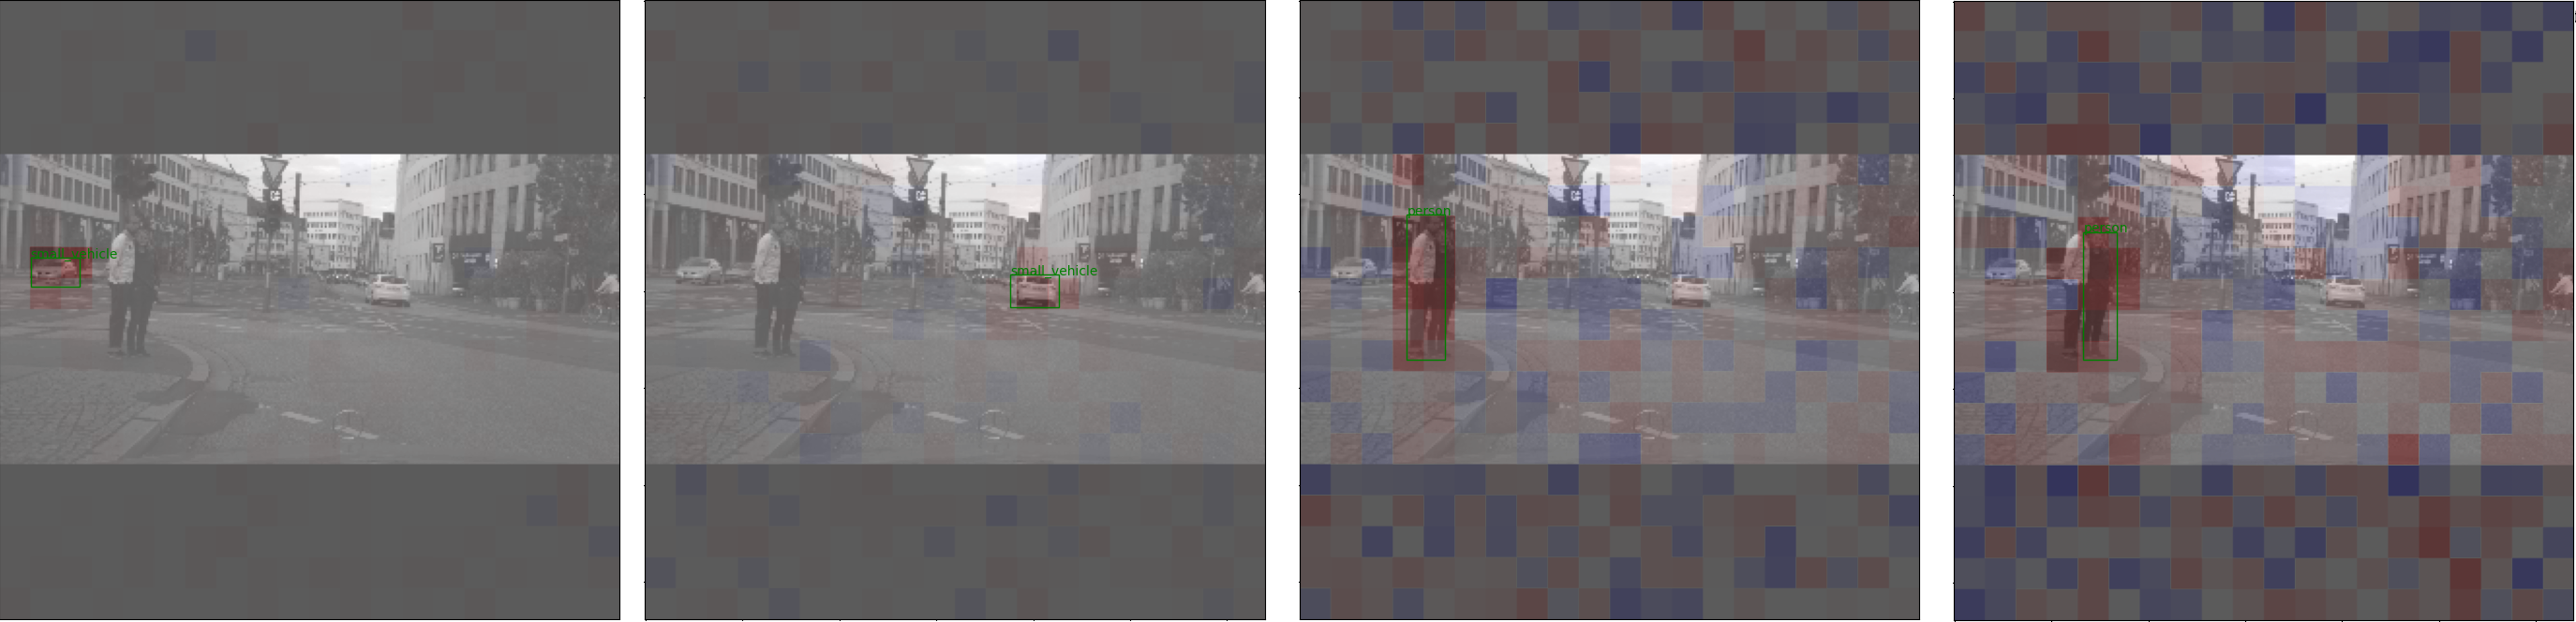
\includegraphics[width=1.0\textwidth]{figures/output1}
\caption{SHAP results for the small vehicle class}\label{fig:SHAP_results1}
\end{figure}
%appliaction of methods

